\documentclass[tikz]{standalone}
\begin{document}
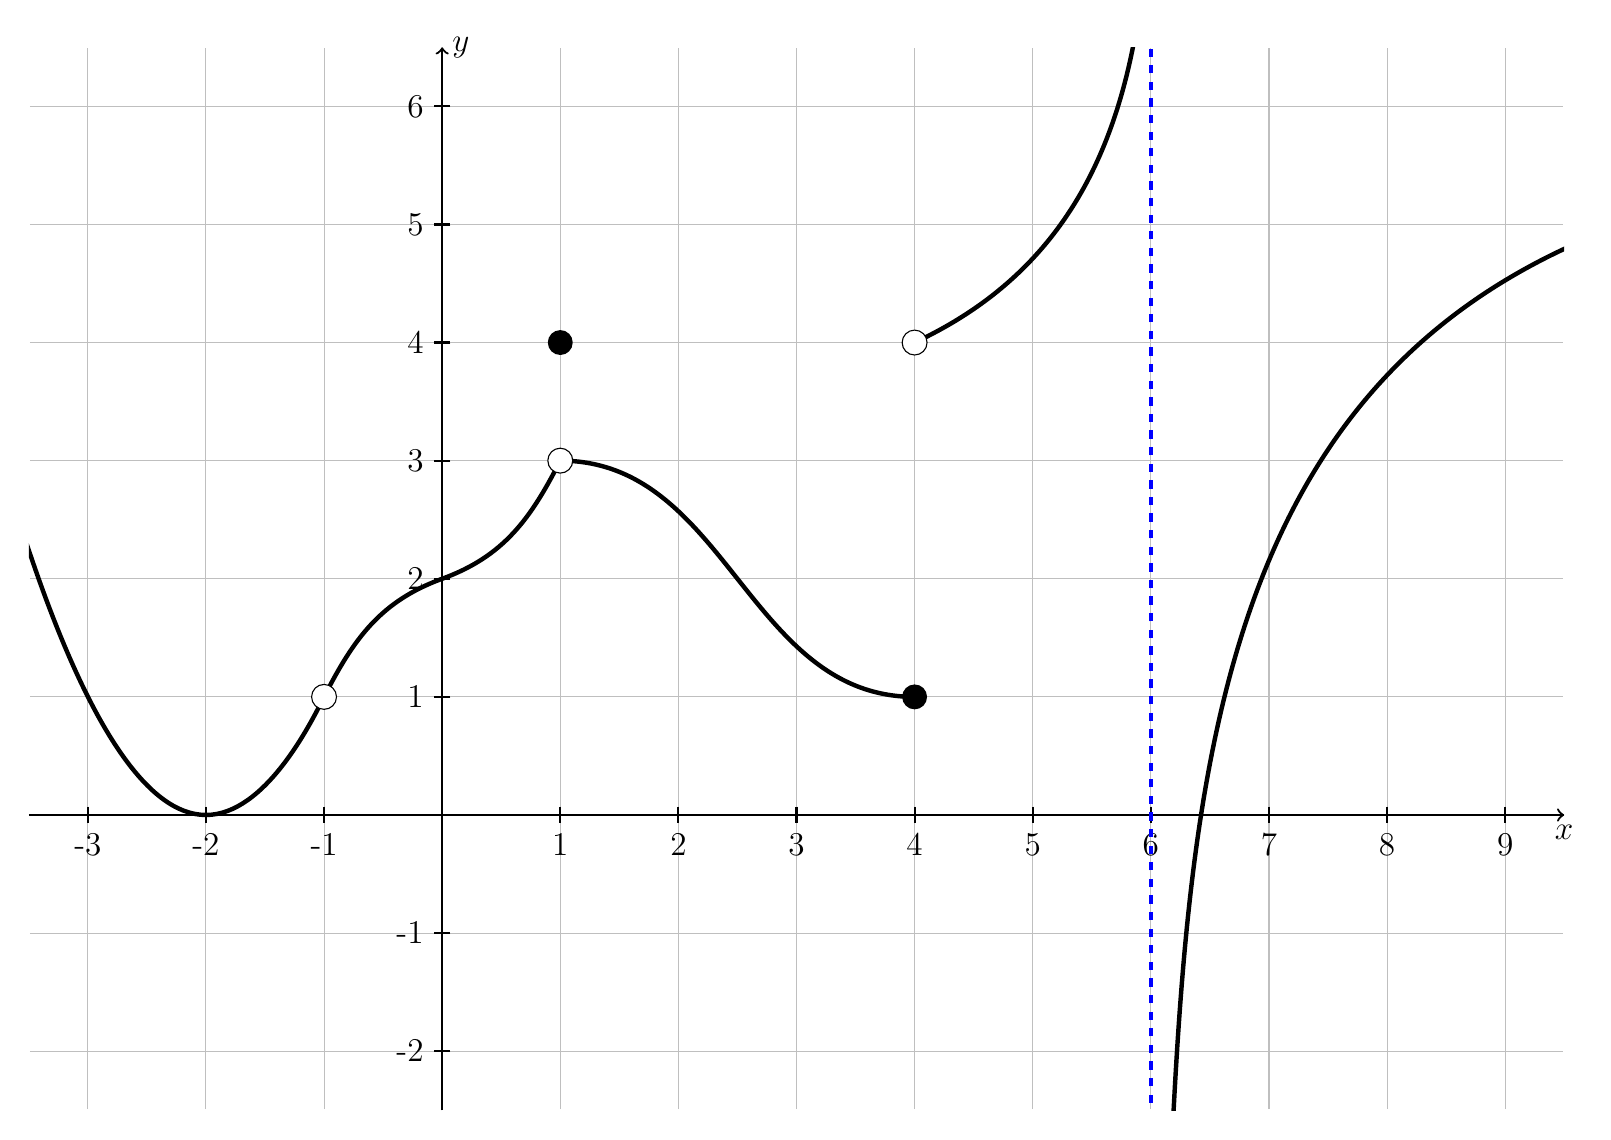
\begin{tikzpicture}[scale=1.5]
\tikzstyle{every node}=[font=\large]

% create a white background, with a black frame
%\draw [fill=white,white] (-4,-3) rectangle (10,7); 

% draw a grid
\draw[step=10mm, lightgray, thin] (-3.49,-2.49) grid (9.49,6.49); 
%\draw[step=1cm, gray] (0,-0) grid (6.5,3.5); 

% draw axes
\draw [->,thick] (-3.5,0) -- (9.5,0) node[below] {$x$}; 
\draw [->,thick] (0,-2.5) -- (0,6.5) node[right] {$y$};

% tick marks
\foreach \x in {-3,-2,...,-1,1,2,...,9} 
	\draw [thick] (\x cm,2pt) -- (\x cm,-2pt) node[below] {\x};
\foreach \y in {-2,-1,1,2,...,6} 
	\draw [thick] (2pt,\y cm) -- (-2pt,\y cm) node[left] {\y};


% plot curve
\clip (-3.5,-2.5) rectangle (9.5,6.5);
\draw [ultra thick,blue,dashed] (6,-3) -- (6,7);
\draw [ultra thick] (-4,4) parabola bend (-2,0) (-1,1);
\draw [ultra thick] (-1,1) to [out=63,in=200] (0,2) to [out=20,in=243] (1,3);
\draw [ultra thick] (1,3) to [out=0,in=180] (4,1);
%\draw[ultra thick,domain=3:1,smooth,samples=300] plot (\x,{2+pow((3-\x)/2,0.33)});
%\draw[ultra thick,domain=3:4,smooth,samples=100] plot (\x,{2-pow(\x-3,0.33)});
\draw [ultra thick] (4,4) to [out=25,in=270] (6,10);
\draw [ultra thick] (6,-6) to [out=85,in=200] (10,5);

% \plot points
\draw [fill=white] (-1,1) circle (3pt);
\draw [fill=white] (1,3) circle (3pt);
\fill (1,4) circle (3pt);
\draw [fill=white] (4,4) circle (3pt);
\fill (4,1) circle (3pt);

\end{tikzpicture}
\end{document}
